\section{结构反事实对比学习}

图~\ref{fig:mechanism} 概括 SC-CL 从训练期候选构造到 Stage~2 联合优化的流程：训练图和训练问题给出可用关系与结构画像，冻结 B1 的训练集分数提供模型违例度；两种信号在已过滤的候选池中混合采样，形成固定的九候选 bank；最后，GRIP Stage~2 联合优化候选损失与原始生成损失。训练期间 bank 只被读取，不根据 valid/test 预测重新采样。测试时按上一节的十选一规则报告官方 EM 与候选排序指标。

\begin{figure}[H]
    \centering
    % Extracted, without resampling, from ../artifacts/结构引导与候选级对比优化流程图.svg.
    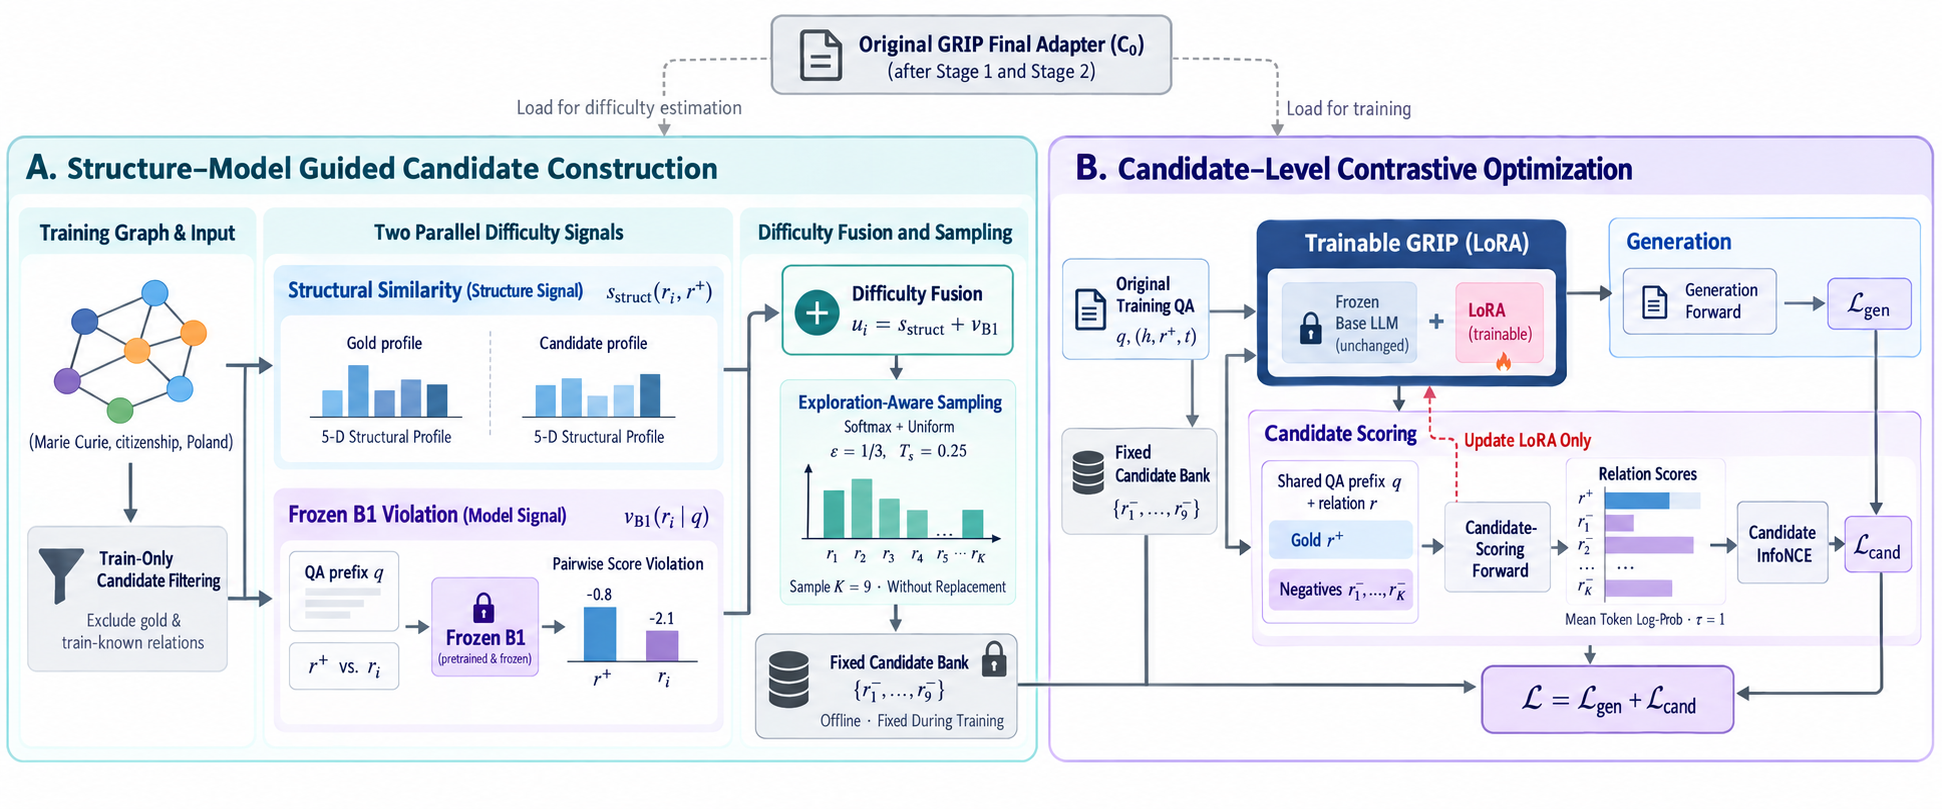
\includegraphics[width=\linewidth]{figures/sccl_structure_guided_svg_content.png}
    \caption{\scc{} 的训练流程。A：训练图关系画像与冻结 \bone{} 分数提供双信号，经过 train-known 过滤与无放回采样，形成每题 $K=9$ 的固定候选库。B：Stage~2 保留原始生成损失，并加入候选级 InfoNCE 共同优化 LoRA。图中损失求和省略了候选权重；严格定义见式~\ref{eq:total}。}
    \label{fig:mechanism}
\end{figure}

图中顶部 $C_0$ 的加载路径为概念性示意：当前实现的 Stage~2 从 Stage~1 adapter 初始化，冻结的 \bone{} 仅用于离线候选评分，不参与训练时的梯度更新。

\subsection{训练图关系画像}

对每一个 $r\in\mathcal{R}_{\mathrm{tr}}$，我们从 $\mathcal{E}_{\mathrm{tr}}$ 计算五维关系画像
\begin{equation}
    \phi(r)=\bigl(\log(1+|E_r|),\log(1+|H_r|),\log(1+|T_r|),
    \overline{d}_{H,r},\overline{d}_{T,r}\bigr),
    \label{eq:profile}
\end{equation}
其中 $|E_r|$ 为关系边数，$|H_r|$ 和 $|T_r|$ 分别为关系覆盖的头实体数与尾实体数，
$\overline{d}_{H,r}$ 是关系边上头实体的平均出度，$\overline{d}_{T,r}$ 是尾实体的平均入度。前两类计数使用 $\log(1+x)$，避免高频关系完全支配距离；度统计保留图的局部连接性。

对目标关系 $r^+$ 和候选 $r$，定义归一化结构相似度
\begin{equation}
    s_{\mathrm{str}}(q,r)=1-\frac{1}{5}\sum_{j=1}^{5}
    \frac{|\phi_j(r^+)-\phi_j(r)|}
    {|\phi_j(r^+)|+|\phi_j(r)|+\epsilon},
    \label{eq:similarity}
\end{equation}
其中 $\epsilon$ 防止两个稀疏特征同时为零。实现将该值裁剪到 $[0,1]$。这个分数只表达“结构画像相近”，不表达两个关系的语义等价性，也不替代对当前实体对的已知关系过滤。

\subsection{冻结 B1 的边界违例度}

\bone{} 是原始 GRIP 的 generation-only 基线。我们在训练问题上离线计算全关系词表的 continuation score。若离线记录已有 pairwise confusion，则直接使用裁剪到 $[0,1]$ 的 confusion；否则对候选和正关系的分数差使用平滑违例度
\begin{equation}
    V_{\bone}(q,r)=\sigma\left(\frac{z_{\bone}(q,r)-z_{\bone}(q,r^+)}{\tau_v}\right).
    \label{eq:violation}
\end{equation}
候选越接近或超过正关系，$V_{\bone}$ 越大。B1 的输出在 bank 构造后冻结，因而 SC-CL 不会把自身训练后的 test 预测反过来用于采样。

\subsection{结构反事实候选分布}

将结构相似度和分数违例度合成为
\begin{equation}
    u(q,r)=\alpha s_{\mathrm{str}}(q,r)+\beta V_{\bone}(q,r),
    \qquad r\in P_q.
    \label{eq:utility}
\end{equation}
候选分布使用均匀下限与 utility softmax 的混合：
\begin{equation}
    p(r\mid q)=\frac{\rho}{|P_q|}+(1-\rho)
    \frac{\exp(u(q,r)/\tau_s)}{\sum_{r'\in P_q}\exp(u(q,r')/\tau_s)}.
    \label{eq:sampling}
\end{equation}
我们从 $p(r\mid q)$ 无放回抽取 $K=9$ 个负关系。默认参数为 $\rho=1/3$、$\alpha=1$、$\beta=1$、$\tau_s=0.25$。如果 $|P_q|<K$，样本进入失败清单而不是静默重复候选；正式实验必须报告该清单及其原因。

这里的“反事实”可写成一个受限操作：在已观测的 $(h,t,r^+)$ 上将标签替换为 $r\in P_q$。$r$ 不是 $T_{\mathrm{tr}}(h,t)$ 中的关系，因此该替换没有复现训练图已知事实；但它仍可能对应真实世界中的未标注事实。这个定义保留了知识图谱的开放世界语义，并让“合法负例”成为数据协议而非未经证实的真值断言。

\subsection{冻结 bank 与候选学习}

SC-CL 的预处理阶段写入每个问题的 question ID、正关系、九个候选、每个候选的结构相似度、违例度、utility、B1 score gap、采样参数、split 和 known-pair 过滤记录。bank manifest 至少满足以下门：

\begin{enumerate}
    \item 所有问题的 \texttt{split} 必须为 \texttt{train}，\texttt{filter\_splits} 只能包含 \texttt{train}；
    \item 每个样本恰有一个正关系和 $K=9$ 个互异候选，候选均属于 $\mathcal{R}_{\mathrm{tr}}$；
    \item 候选与 $T_{\mathrm{tr}}(h,t)$ 不相交，且 question ID 与完整 task JSON 一一对齐；
    \item bank hash、脚本版本、随机种子和结构采样参数被写入 manifest，训练后不得覆盖原文件。
\end{enumerate}

训练时，候选 continuation score 代入式~\ref{eq:infonce}，生成损失仍按原始 GRIP 路径计算。该设计将 SC-CL 的影响集中到“给定候选集合如何区分关系”，而不是同时改变上下文构造或自由解码。

\subsection{复杂度与实现边界}

关系画像只需一次线性扫描训练边，复杂度为 $O(|\mathcal{E}_{\mathrm{tr}}|)$；每个问题的候选 utility 在关系词表上计算，复杂度约为 $O(|\mathcal{R}_{\mathrm{tr}}|)$，采样后 bank 大小为 $O(K|Q_{\mathrm{tr}}|)$。结构画像与采样本身不需要 GPU；冻结 B1 的全关系 continuation scoring 和后续候选训练则需要额外模型计算，实测成本见第 5 节。确定性、过滤和非训练 split 拒绝通过实现测试检查。
